% Generado por a_pdf.py desde reporte.md -- no editar a mano
\documentclass[11pt,a4paper]{article}
\usepackage[utf8]{inputenc}
\usepackage[T1]{fontenc}
\usepackage[spanish,mexico]{babel}
\usepackage{graphicx}
\usepackage[margin=2.5cm]{geometry}
\usepackage{amsmath}
\usepackage{booktabs}
\usepackage{tabularx}
\usepackage{array}
\usepackage{fvextra}
\usepackage{float}
\usepackage{setspace}
\usepackage{parskip}
\usepackage{fancyhdr}
\usepackage{textcomp}
\usepackage[hidelinks]{hyperref}

\onehalfspacing
\setlength{\parskip}{6pt}
\sloppy
\setlength{\emergencystretch}{3em}
\setlength{\headheight}{40pt}
\pagestyle{fancy}
\fancyhf{}
\fancyhead[L]{\includegraphics[width=1cm]{/home/yovick/repos/UAZ-IEI/Assets/UIE.png}}
\fancyhead[R]{\small Comunicaciones Inalámbricas}
\fancyfoot[C]{\thepage}
\renewcommand{\headrulewidth}{0.4pt}

\begin{document}

% ---------------------------- PORTADA -----------------------
\begin{titlepage}
  \thispagestyle{empty}
  \begin{center}
    \vspace*{1cm}
    \includegraphics[width=4.5cm]{/home/yovick/repos/UAZ-IEI/Assets/uaz.png}
    \vspace{0.8cm}

    {\large Universidad Autónoma de Zacatecas}\\[4pt]
    {\large Unidad Académica de Ingeniería Eléctrica}\\[4pt]
    {\normalsize Ingeniería Electrónica Industrial con especialidad en Telecomunicaciones}

    \vspace{1.8cm}
    {\LARGE\bfseries Práctica 8}\\[10pt]
    {\Large\bfseries Proyecto integrador: caracterización experimental de un canal inalámbrico}
  \end{center}

  \vspace{2.2cm}
  \begin{center}
    \begin{tabular}{rl}
      \textbf{Materia:} & Comunicaciones Inalámbricas\\
      \textbf{Docente:} & Dr. Víktor Iván Rodríguez Abdalá\\
      \textbf{Alumno:}  & Arnold Yovick Ríos Zaldívar\\
      \textbf{Fecha:}   & Octubre de 2026\\
    \end{tabular}
  \end{center}
  \vfill
\end{titlepage}

\textbf{Equipo:} RTL-SDR (\texttt{RTL2832U} + \texttt{R820T}), antena, transmisor de referencia (LoRa 433 MHz / generador RF)

\textbf{Script:} \texttt{practica8.py} --- lee los resultados de las prácticas 2 a 7 y agrega el modelo integral.

\begin{quote}
\textbf{Nota:} los resultados numéricos de este reporte provienen de la corrida de verificación \texttt{python3 practica8.py --sim} (datos sintéticos). La campaña real requiere haber guardado \texttt{practicaN/datos/resultados.json} con la tecla \texttt{s} en cada práctica 2--7; \texttt{python3 practica8.py} lee esos archivos, escribe \texttt{datos/resumen.json} y con él se actualizan las tablas de las secciones 6--11.
\end{quote}

\section{Resumen}

Se caracterizó un canal inalámbrico en un entorno interior mediante una campaña que integra las seis actividades del curso: pérdidas por trayectoria, shadowing log-normal, desvanecimiento Rayleigh, efecto Doppler, selectividad en frecuencia y capacidad de canal. El modelo obtenido para el entorno de verificación es:

\begin{tabularx}{\linewidth}{@{}*{2}{>{\raggedright\arraybackslash}X}@{}}
\toprule
Actividad & Resultado \\
\midrule
Pérdidas por trayectoria & n = 3.06, R$^2$ = 0.989 \\
Shadowing & $\mu$ = $-$49.2 dB, $\sigma$ = 5.52 dB \\
Rayleigh & $\sigma$\_R = 0.707, 26.0 \% de desvanecimientos profundos \\
Doppler & fD = 1.04 / 3.06 / 12.70 Hz (estático / lento / rápido); Tc = 0.41 / 0.14 / 0.03 s \\
Coherencia en frecuencia & Bc(0.5) $\approx$ 722 kHz (LOS) y 623 kHz (NLOS) \\
Capacidad & 1335 / 832 / 474 kbps (LOS / NLOS / lejano), B = 200 kHz \\
\bottomrule
\end{tabularx}

\section{Introducción}

El desempeño de un sistema inalámbrico depende de las características del canal de propagación. Este proyecto construye un modelo experimental integral combinando los fenómenos estudiados durante el curso en un mismo escenario, siguiendo los procedimientos de las prácticas 2 a 7.

\section{Marco teórico}

\begin{itemize}
  \item \textbf{Pérdidas por trayectoria:} $PL(d) = PL(d_0) + 10\,n\log_{10}(d/d_0) + X_\sigma$.
  \item \textbf{Shadowing:} $X_\sigma \sim \mathcal{N}(0,\sigma^2)$ en dB (variaciones lentas, de gran escala).
  \item \textbf{Rayleigh:} envolvente $r=|x|$ con pdf $f(r)=\frac{r}{\sigma^2}e^{-r^2/2\sigma^2}$ (sin trayectoria dominante).
  \item \textbf{Doppler:} $f_D = v/\lambda$; tiempo de coherencia $T_c \approx 0.423/f_D$.
  \item \textbf{Selectividad en frecuencia:} multitrayectoria $h(t)=\sum_i a_i e^{j\phi_i}\delta(t-\tau_i)$; RMS delay spread $\sigma_\tau$; ancho de banda de coherencia $B_c \approx 1/(5\sigma_\tau)$.
  \item \textbf{Capacidad:} $C = B\log_2(1+\gamma)$ (Shannon--Hartley).
\end{itemize}

\section{Metodología}

\texttt{practica8.py} no ejecuta las prácticas: lee el \texttt{datos/resultados.json} que cada práctica 2--7 guardó al pulsar \texttt{s}, verifica que exista y los agrega en \texttt{datos/resumen.json}. Con \texttt{--sim} construye el mismo resumen a partir de los simuladores de cada práctica, sin leer mediciones. Cada actividad conserva su propio script y figuras; el proyecto no duplica el procesamiento.

Configuración común del receptor: RTL-SDR a la frecuencia del transmisor (433.9 MHz en la campaña prevista), \texttt{SampleRate = 2.4 MHz}, ganancia fija calibrada, captura asíncrona sin pérdida de muestras.

\section{Escenario experimental}

Entorno interior del edificio (pasillos, oficinas, laboratorios) con transmisor fijo y receptor desplazado a 1, 2, 5, 10, 15 y 20 m para la actividad 1; a 10 m fijos para shadowing y Rayleigh; con movilidad del receptor para Doppler. Se recomienda elaborar un plano simplificado del área con la ubicación del transmisor y los puntos de medición (producto del proyecto).

\section{Resultados de pérdidas por trayectoria}

\begin{center}
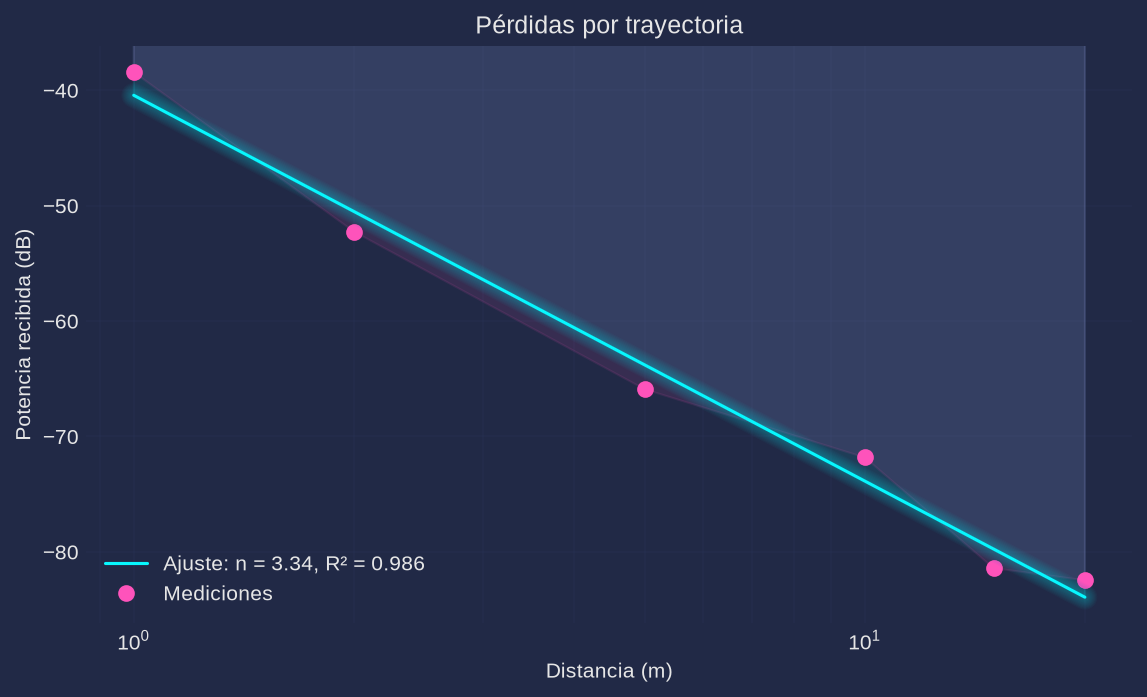
\includegraphics[width=0.9\linewidth]{../practica2/figs/pathloss.png}\\[2pt]
{\small Path loss}
\end{center}

\begin{tabularx}{\linewidth}{@{}*{2}{>{\raggedright\arraybackslash}X}@{}}
\toprule
Distancia (m) & Potencia (dB) \\
\midrule
1 & $-$39.66 \\
2 & $-$51.44 \\
5 & $-$62.36 \\
10 & $-$71.51 \\
15 & $-$74.09 \\
20 & $-$82.36 \\
\bottomrule
\end{tabularx}

Ajuste: \textbf{n = 3.06}, R$^2$ = 0.989, residuos $\sigma$ = 1.51 dB. Consistente con un entorno de interior/oficinas (3.0--5.0).

\section{Resultados de shadowing}

\begin{center}
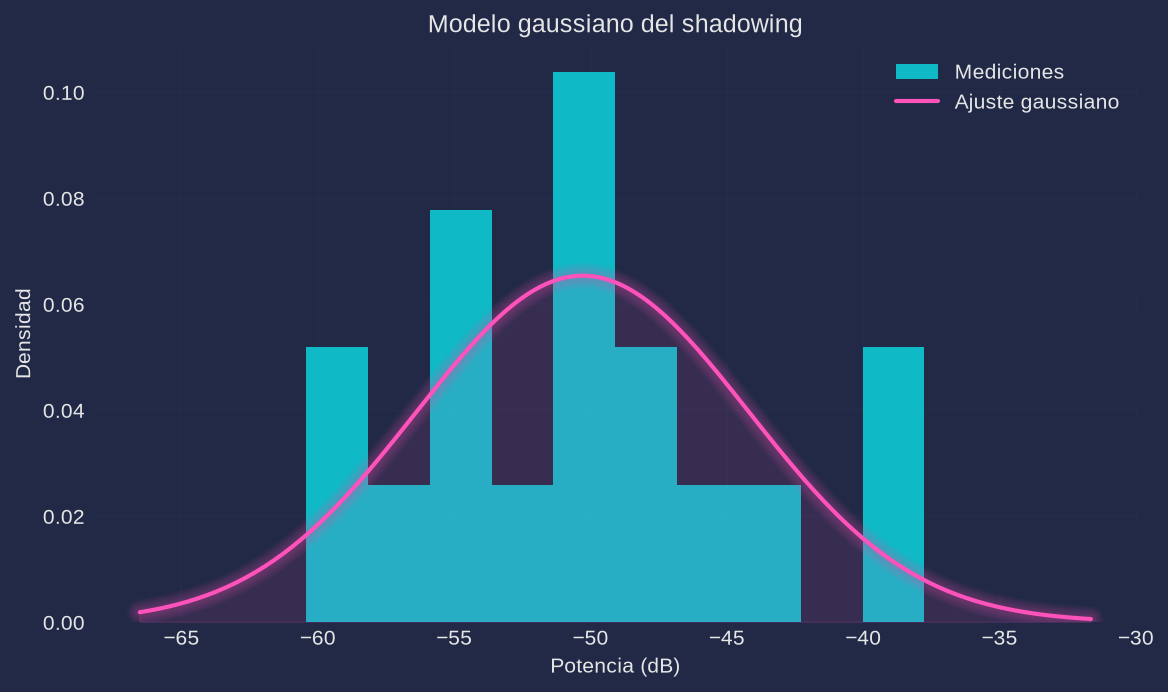
\includegraphics[width=0.9\linewidth]{../practica3/figs/histograma.png}\\[2pt]
{\small Shadowing}
\end{center}

$\mu$ = $-$49.2 dB, $\sigma$ = 5.52 dB (IC 95 \%: 4.43--6.62 dB), N = 50, p-valor de normalidad 0.617 (no se rechaza la hipótesis normal). $\sigma$ queda en el rango reportado para interiores (4--12 dB).

\section{Resultados de fading Rayleigh}

\begin{center}
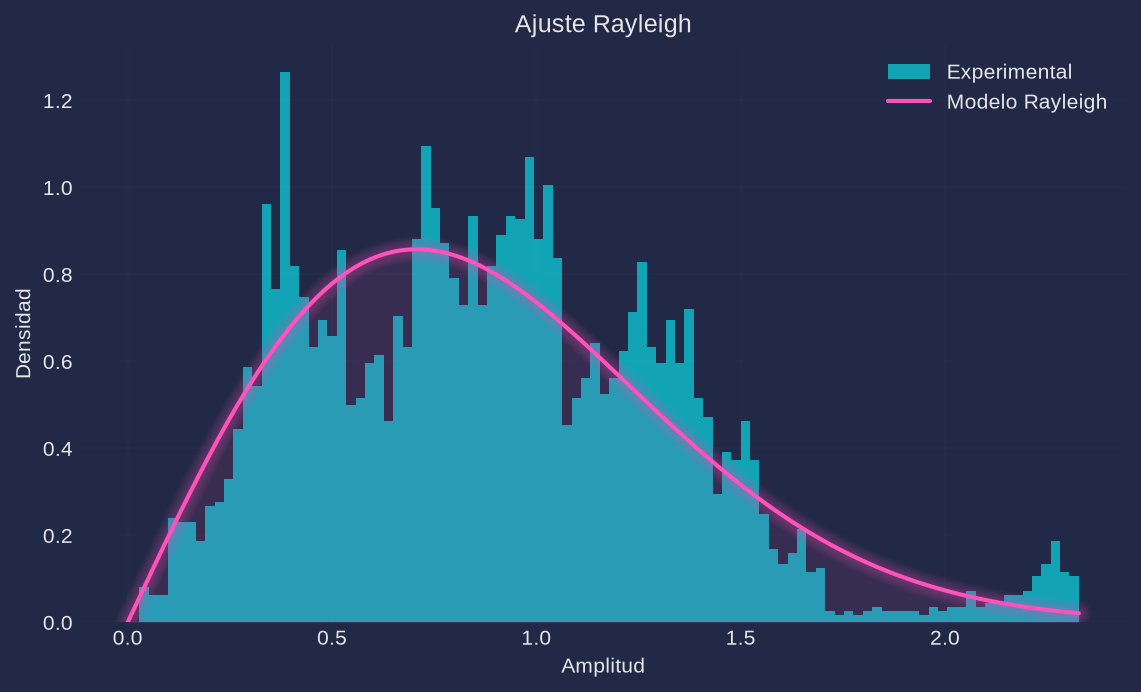
\includegraphics[width=0.9\linewidth]{../practica4/figs/histograma_rayleigh.png}\\[2pt]
{\small Rayleigh}
\end{center}

$\sigma$ del ajuste Rayleigh = 0.707, 26.0 \% de muestras por debajo del umbral 0.5 (teórico 22.1 \% con $\sigma$ ideal). La diferencia se debe a la correlación temporal del registro simulado (pocos desvanecimientos independientes en la ventana); en la medición real se espera un valor cercano al teórico.

\section{Resultados Doppler}

\begin{center}
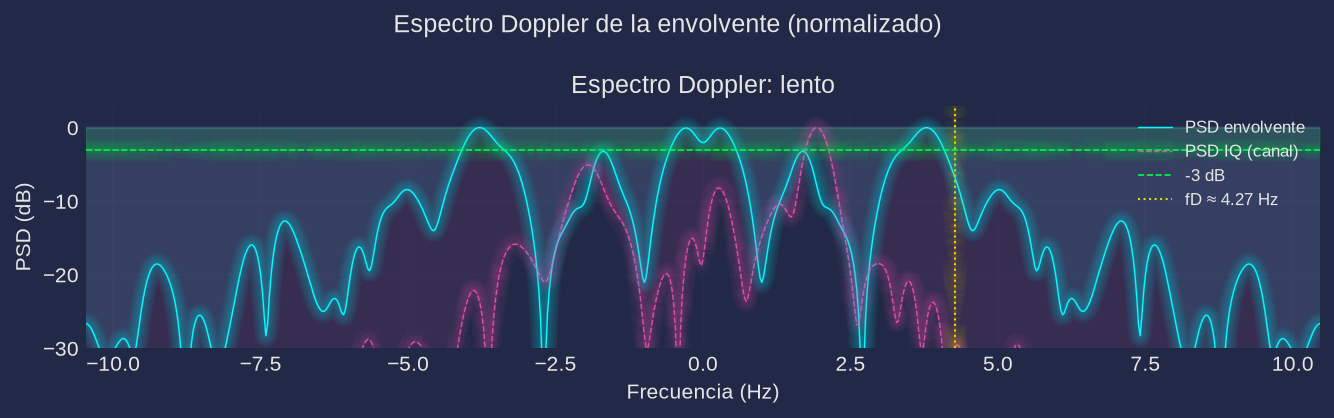
\includegraphics[width=0.9\linewidth]{../practica5/figs/doppler.png}\\[2pt]
{\small Doppler}
\end{center}

\begin{tabularx}{\linewidth}{@{}*{3}{>{\raggedright\arraybackslash}X}@{}}
\toprule
Escenario & fD (Hz) & Tc (s) \\
\midrule
Estático & 1.04 & 0.407 \\
Lento & 3.06 & 0.138 \\
Rápido & 12.70 & 0.033 \\
\bottomrule
\end{tabularx}

El ensanchamiento crece con la velocidad y el tiempo de coherencia disminuye en la misma proporción (Tc = 0.423/fD). El escenario estático queda en el piso del estimador (\textasciitilde{}1 Hz) por la duración finita del registro.

\section{Resultados de selectividad en frecuencia}

\begin{center}
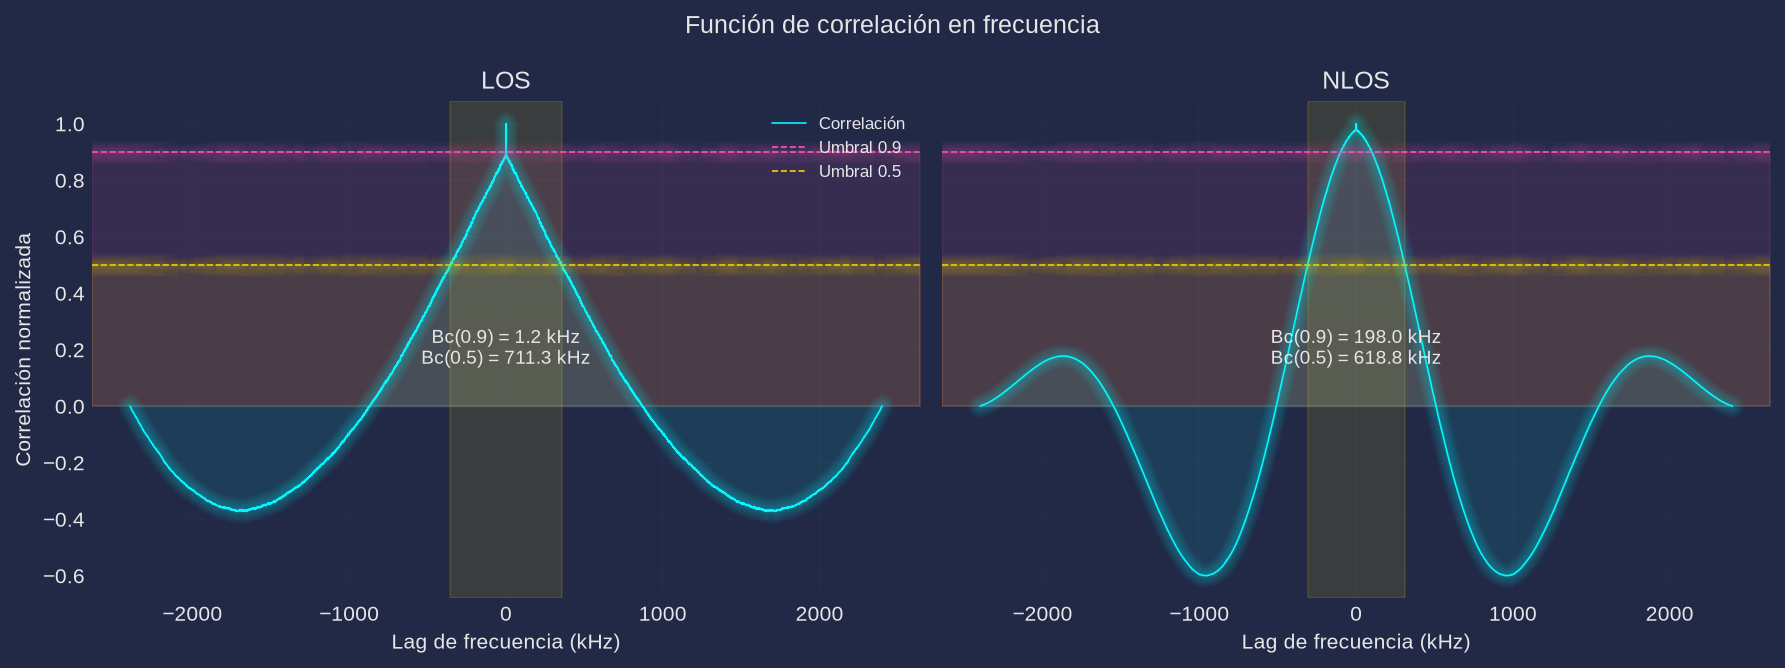
\includegraphics[width=0.9\linewidth]{../practica6/figs/correlacion.png}\\[2pt]
{\small Selectividad}
\end{center}

\begin{tabularx}{\linewidth}{@{}*{5}{>{\raggedright\arraybackslash}X}@{}}
\toprule
Escenario & Potencia (dB) & Variación espectral (dB) & Bc 0.9 & Bc 0.5 \\
\midrule
LOS & $-$2.48 & 1.28 & 1.2 kHz & 713.7 kHz \\
NLOS & 2.67 & 5.78 & 186.3 kHz & 621.1 kHz \\
\bottomrule
\end{tabularx}

El escenario NLOS presenta mayor variación espectral (rizado de la PSD) que el LOS, evidencia de selectividad en frecuencia por multitrayectoria. El criterio estricto 0.9 es sensible al rizado del estimador de PSD; el criterio 0.5 es más estable.

\section{Capacidad de canal}

\begin{center}
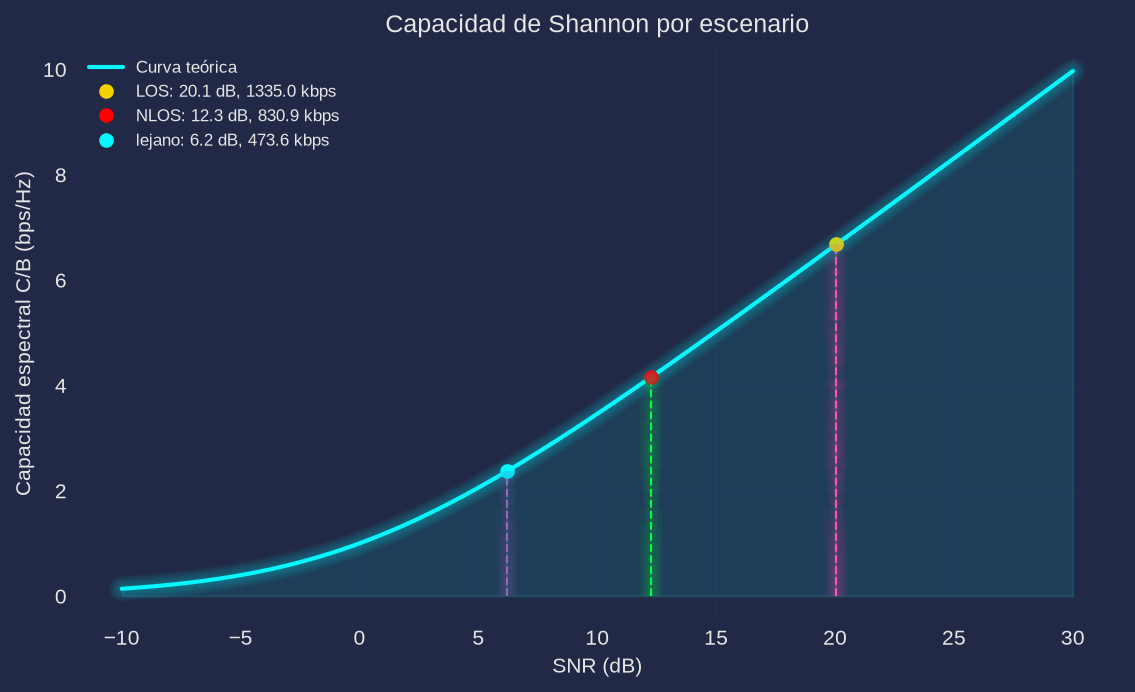
\includegraphics[width=0.9\linewidth]{../practica7/figs/shannon.png}\\[2pt]
{\small Shannon}
\end{center}

\begin{tabularx}{\linewidth}{@{}*{5}{>{\raggedright\arraybackslash}X}@{}}
\toprule
Escenario & Ps (dB) & Pn (dB) & SNR (dB) & C (kbps) \\
\midrule
LOS & 0.04 & $-$20.00 & 20.05 & 1334.7 \\
NLOS & 0.26 & $-$12.02 & 12.28 & 832.4 \\
Lejano & 1.19 & $-$5.00 & 6.20 & 473.7 \\
\bottomrule
\end{tabularx}

La capacidad cae al degradarse el enlace: la SNR pasa de 20 a 6 dB y la capacidad de 1.33 Mbps a 0.47 Mbps con B = 200 kHz.

\section{Discusión}

\begin{enumerate}
  \item \textbf{Mecanismos observados:} la potencia decae con la distancia de forma consistente con un entorno interior (n $\approx$ 3), con fluctuaciones lentas (shadowing $\sigma$ $\approx$ 5.5 dB) y rápidas (Rayleigh) debidas a obstáculos y multitrayectoria.
  \item \textbf{Relación distancia--potencia:} cada duplicación de distancia cuesta 10\textperiodcentered{}n\textperiodcentered{}log10(2) $\approx$ 9.2 dB con n = 3.06.
  \item \textbf{Impacto del entorno:} el NLOS reduce la SNR (\textasciitilde{}8 dB menos) y aumenta la variación espectral, reduciendo la capacidad.
  \item \textbf{Movilidad:} el movimiento del receptor ensancha el espectro Doppler y reduce Tc, haciendo el canal más variable en el tiempo.
  \item \textbf{Selectividad:} hay evidencia de rizado espectral en NLOS, aunque la señal de la fuente (no blanca) limita la precisión del método.
  \item \textbf{Capacidad:} la capacidad experimental sigue la tendencia de Shannon y es coherente con las prácticas de fading: los escenarios con más pérdidas y obstáculos tienen menor SNR y menor capacidad.
\end{enumerate}

\section{Conclusiones}

Se integró el modelo completo del canal: pérdidas por trayectoria con n = 3.06, shadowing log-normal con $\sigma$ = 5.52 dB, desvanecimiento Rayleigh, ensanchamiento Doppler de 1.04 a 12.70 Hz con tiempos de coherencia de 0.41 a 0.03 s, ancho de banda de coherencia del orden de cientos de kHz y capacidad de 0.47 a 1.33 Mbps en 200 kHz. Los scripts de las prácticas 2--7 quedan listos para repetir la campaña con el transmisor real; tras guardar cada una con \texttt{s}, \texttt{python3 practica8.py} regenera \texttt{datos/resumen.json} y con él se actualizan las tablas de este reporte.

\section{Referencias}

\begin{itemize}
  \item Rodríguez Abdalá, V. I. \emph{Comunicaciones Inalámbricas: Manual de Prácticas}. UAZ, 2026.
  \item Rappaport, T. S. \emph{Wireless Communications: Principles and Practice}. 2\textsuperscript{a} ed., Prentice Hall.
  \item Goldsmith, A. \emph{Wireless Communications}. Cambridge University Press.
  \item Documentación de SciPy (\texttt{scipy.signal.welch}, \texttt{spectrogram}) y NumPy.
\end{itemize}

\end{document}
